\lecture{18}{05.09}
\begin{notation}
    经过QMF的离子呈螺线前进
\end{notation}
4.4. 飞行时间质量分析器TOF:使用电压加速带电粒子,通过公式:\[
    \frac{1}{2}mv^2 = zU
.\]
计算飞行速度和飞行时间:
\[
    v = \sqrt{\frac{2Uze}{m}} \quad t = \frac{L}{v}
.\]
一般来说,质荷比$m / z$ 越大,飞行时间越长
\begin{notation}
    不同质荷比的离子到达终点的时间差:
    \[
        \Delta t = L \frac{\sqrt{\left( m / z \right)_1}-\sqrt{\left( m / z \right)_2}}{\sqrt{2U}}
    .\]
\end{notation}
4.5. 离子阱,原理类似QMF,使用环形电极来加速离子,使目标离子进入特定轨道,其他离子撞击环电极
\subsubsection{检测系统}%
\label{ssub*:检测系统}
常用的有\textbf{法拉第杯、电子倍增管、微通道板、闪烁计数器};作用为接受质量分析器的离子并计数,转换为质谱图
\subsection{质谱仪主要性能指标}%
\label{sub:质谱仪主要性能指标}
\begin{enumerate}
    \item 质量范围:$\Delta\left( m / z \right)$
    \item 分辨率:如果两个相等强度的峰强度重合的部分不大于10\%,就认为可以分辨这两个质量数
    \item 灵敏度:仪器出峰的强度和所用样品之间的关系
    
\end{enumerate}
\begin{defi}
    \[
    1\text{amu} = 1.66053906660 \times 10^{-27} \ce{kg}
    .\]
    即$\ce{^12C}$ 质量的$1 / 12$
\end{defi}
\begin{notation}
    四极杆质谱仪的质量范围一般在10-1000amu,磁质谱仪一般为1-10000amu,飞行时间质谱仪无上限
\end{notation}
\begin{notation}
仪器的分辨率:\[
    R = \frac{m_1}{m_2-m_1} = \frac{m_1}{\Delta m}
.\]
其中$m_1<m_2$
\end{notation}
当$R>1000$ 时称为高分辨率
\begin{eg}
    $\left( m / z \right)_{\ce{N_2+}} = 28.0061, \left( m / z \right)_{\ce{CO+}} = 27.9949$ ,如果要区分这两种离子,需要分辨率达到:\[
        R > \frac{27.9949}{28.0061-27.9949} = 2499.545
    .\]
\end{eg}
\begin{notation}
    飞行时间质谱要求提供半峰分辨率
\end{notation}
\begin{notation}
    灵敏度一般定义为:一定分辨率下产生一定信噪比S/N所需的进样量
\end{notation}
\subsection{质谱的表示}%
\label{sub:质谱的表示}
以质荷比$m / z$ 为横坐标,相对强度为纵坐标,将最强的峰定为基峰,强度定义为100\%;其他的离子通过基峰的含量占比表示
\begin{figure}[htpb]
    \centering
    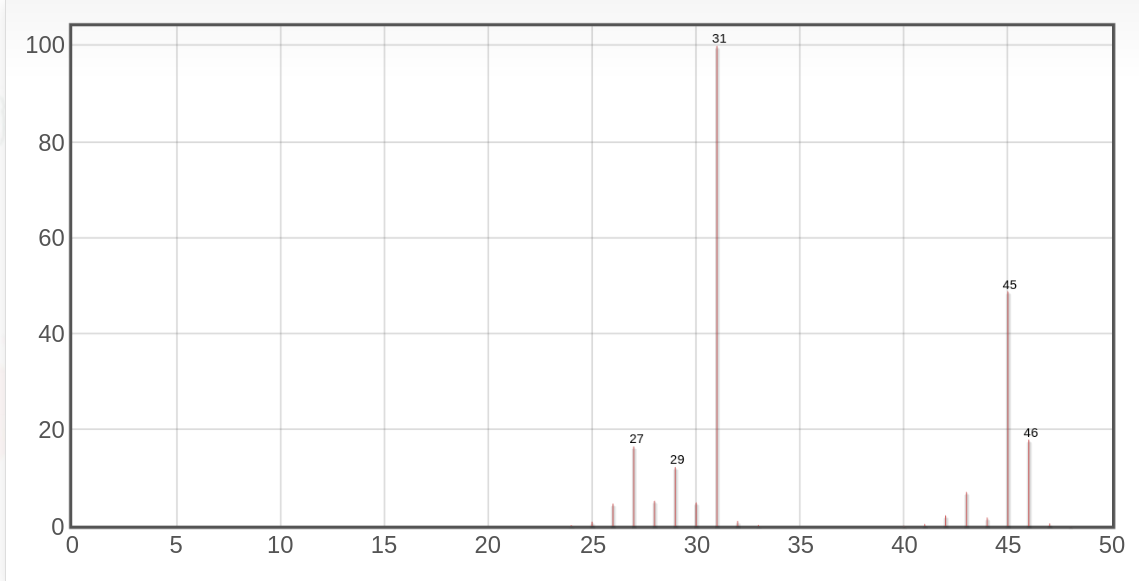
\includegraphics[width=0.8\textwidth]{./figures/乙醇质谱图.png}
    \caption{乙醇质谱图,图片来源:上海有机所专业数据库}
    \label{fig:-figures-乙醇质谱图-png}
\end{figure}
图中的组成:
\subsubsection*{分子离子}%
\label{subsub*:分子离子}
\[
    \ce{M + e- \to M^{+.} + 2e-}
.\]
分子离子的$z = 1, m / z = m$ ,即最大质荷比的位置即为该分子的分子量
\subsubsection*{碎片离子}%
\label{subsub*:碎片离子}
分子离子裂解为初级碎片离子,初级碎片离子继续裂解或重排为次级碎片离子
\begin{eg}
    对于丙酮$\ce{CH_3C(=O)CH_3}$ ,其分子离子为$\ce{CH_3C(=O+)CH_3}, m / z = 58$ ,第一次裂解为$\ce{CH_3C#O+}, m / z = 43$,第二次裂解为$\ce{CH_3+}, m / z = 15$ 
    \begin{figure}[htpb]
        \centering
        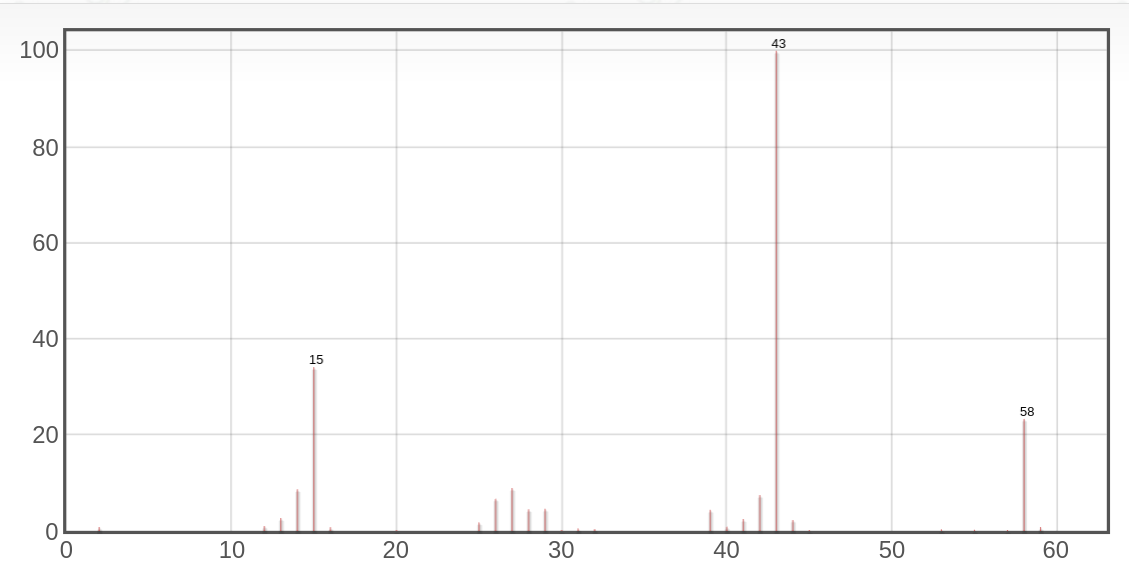
\includegraphics[width=0.8\textwidth]{./figures/丙酮质谱图.png}
        \caption{丙酮质谱图}
        \label{fig:-figures-丙酮质谱图-png}
    \end{figure}
\end{eg}
\subsubsection*{亚稳离子}%
\label{subsub*:亚稳离子}
在飞行过程中失去了一部分中性碎片的质量,有一部分能量被带走,此时的离子的质量小,能量低,不稳定,用$m^\star $ 表示
\begin{notation}
    一般$m^\star $ 的质荷比不是整数
\end{notation}
\begin{figure}[htpb]
    \centering
    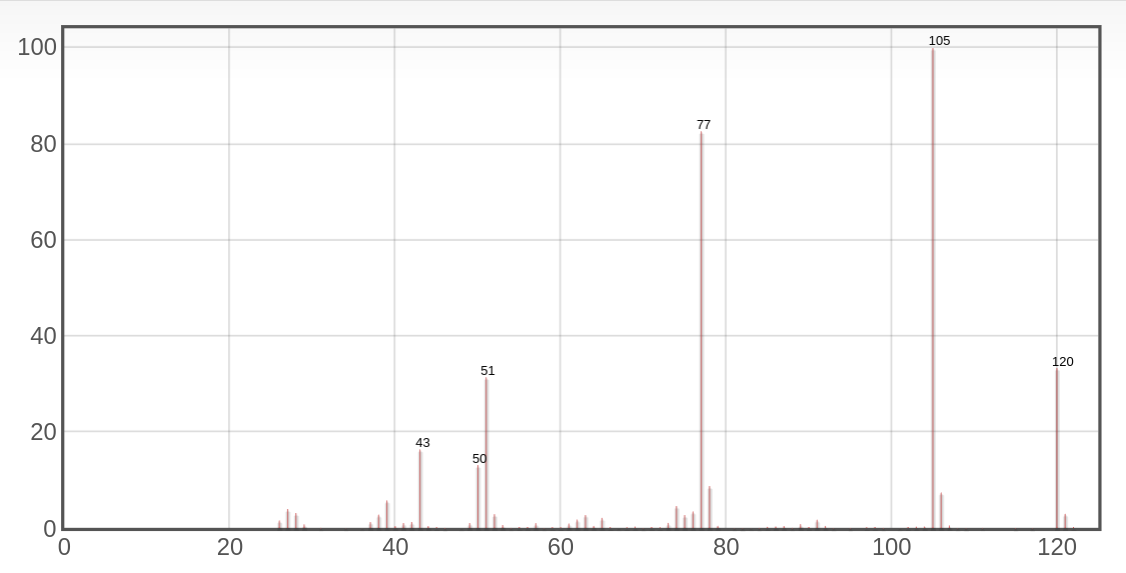
\includegraphics[width=0.8\textwidth]{./figures/苯乙酮质谱.png}
    \caption{苯乙酮质谱图}
    \label{fig:-figures-苯乙酮质谱-png}
\end{figure}
\subsubsection*{同位素离子}%
\label{subsub*:同位素离子}
在质谱图上体现为$M+1, M+2$ 的峰,原因为不同的同位素质量数相差1到2
\begin{notation}
    阳离子的裂解:单纯开裂和重排开裂,失去电子的难易程度:$n>\pi>\sigma$

    均裂:成键电子被每个碎片各拿一个
    \begin{eg}
        含双键的化合物$\sigma$ 均裂:
        \[
        \ce{R_1-C(=X^{+.})-R_2 \to R_1-C#X^+ + R_2^.}
        .\]
    \end{eg}
    异裂:两个成键电子都属于某一个碎片
    \begin{eg}
        如果R1>R2,遵循\textbf{最大烷基丢失原则}:
        \[
        \ce{R_1-C(=X^{+.})-R_2 \to R_1-C#X^{+.} + R_2^+}
        .\]
    \end{eg}
    半异裂:已经离子化的$\sigma$ 键中仅存的一个电子转移到另一个碎片上
    \begin{eg}
        游离的烷基发生半异裂:\[
            \ce{R-(CH_2^{+.})-CH_2CH_3 \to R-CH_2^{+} + ^.CH_2CH_3}
        .\]
    \end{eg}
\end{notation}
\begin{notation}
    $\alpha$ 裂解:分子中含有$\ce{C-X}$ 或$\ce{C=X}$ ,其中X可以是C, O, S, Cl等,这个键旁边的键称为 $\alpha$ 键,断裂后,两个原子的电子可以形成新的双键/三键,称为$\alpha$ 裂解

    苄基断裂:经过$\alpha$ 裂解后再重排为稳定的苄基基团,该基团一般会是整个谱图中的最强峰($m / z = 91$, 图\ref{fig:-figures-乙苯质谱图-png})
    \begin{figure}[htpb]
        \centering
        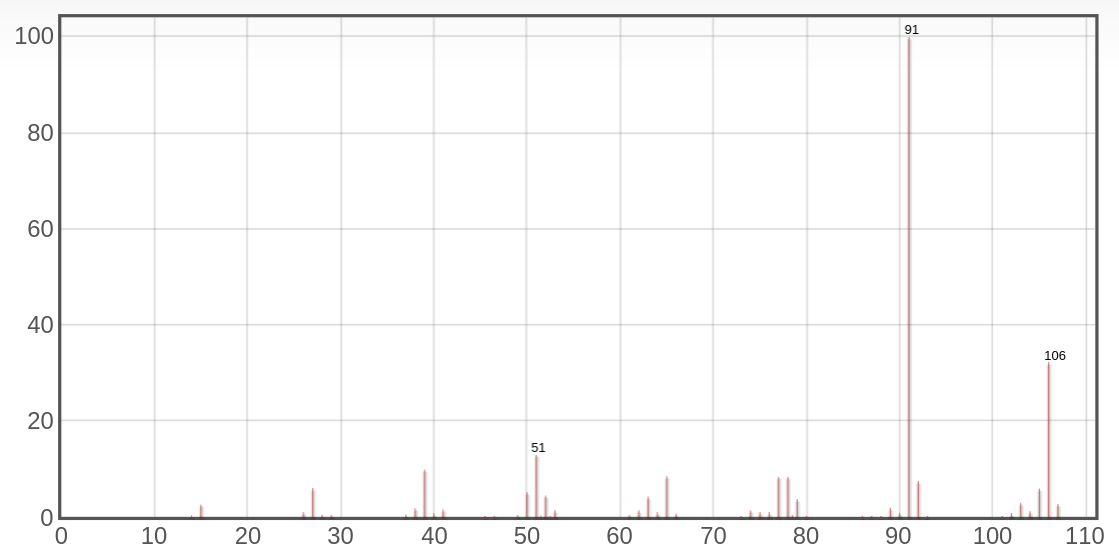
\includegraphics[width=0.8\textwidth]{./figures/乙苯质谱图.png}
        \caption{乙苯质谱图}
        \label{fig:-figures-乙苯质谱图-png}
    \end{figure}
    
    同理,烯丙基的裂解会产生一个$m / z = 41$ 的基峰(图\ref{fig:-figures-丙烯质谱图})
    \begin{figure}[htpb]
        \centering
        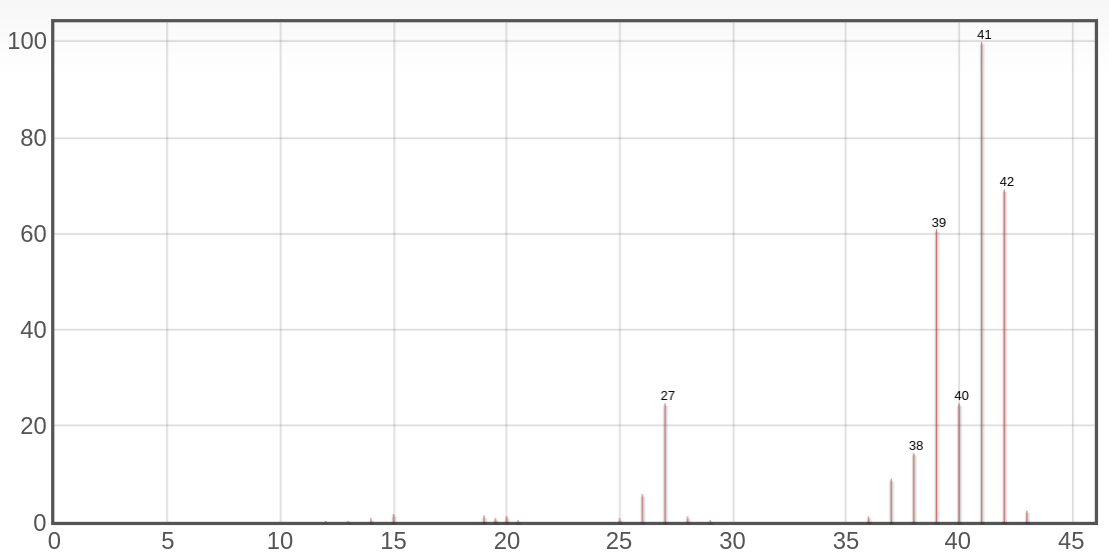
\includegraphics[width=0.8\textwidth]{./figures/丙烯质谱图}
        \caption{丙烯质谱图}
        \label{fig:-figures-丙烯质谱图}
    \end{figure}
\end{notation}
\begin{notation}
    重排开裂:分为麦氏重排和狄尔斯阿尔德重排

    麦氏重排:含有C=O, C=N, C=S, C=C,通过一个六元环体系将$\gamma$-H原子转移到X原子上,同时发生$\beta$ 键断裂
\end{notation}
